% $Date: 2022/12/30 17:24:03 $
% This template file is public domain.
%
% TUGboat class documentation is at:
%   http://mirrors.ctan.org/macros/latex/contrib/tugboat/ltubguid.pdf
% or
%   texdoc tugboat

\documentclass[twocolumn,10pt]{article}
\setlength{\columnsep}{.3in}
\setlength{\columnseprule}{.5pt}
\pagestyle{empty}

\usepackage{listings}
\usepackage{tikz}
\usepackage{amsmath, amssymb}
\usepackage{microtype}
\usepackage{graphicx}
\usepackage{array, float}
\usepackage{caption}
\usepackage{enumerate}
\usepackage[hidelinks,pdfa]{hyperref}
\usepackage[a4paper, total={7.5in, 9.2in}, vcentering]{geometry}

\usepackage{fancyhdr} % 导入fancyhdr包
\pagestyle{fancy}
% 页眉设置
\fancyhead[C]{Numerical PDE Homework \# 5}
\fancyhead[R]{May 24, 2023}
\fancyhead[L]{Wenchong Huang}
\fancyfoot[C]{\thepage} % 页码

%%% Start of metadata %%%

% repeat info for each author; comment out items that don't apply.
%\ORCID{0}
% To receive a physical copy of the TUGboat issue, please include the
% mailing address we should use, as a comment if you prefer it not be printed.

%%% End of metadata %%%

\begin{document}

\section*{\large Exercise 12.11}

 By (12.11) and (12.19), for $i=2,...,m-1$ we have
\begin{align*}
    & \left[\left(I-\frac{k}{2}A\right)\mathbf{U}^{n+1}\right]_i\\
    =& -\frac{k\nu}{2h^2}U_{i-1}^{n+1} + \left(1+\frac{k\nu}{h^2}\right)U_i^{n+1} - \frac{k\nu}{2h^2}U_{i+1}^{n+1}\\
    =& -\frac{r}{2}U_{i-1}^{n+1} + \left(1+r\right)U_i^{n+1} - \frac{r}{2}U_{i+1}^{n+1}\\
    =& \frac{r}{2}U_{i-1}^{n} + \left(1-r\right)U_i^{n} + \frac{r}{2}U_{i+1}^{n}\\
    =& \left[\left(I+\frac{k}{2}A\right)\mathbf{U}^{n}\right]_i\\
    =& \left[\left(I+\frac{k}{2}A\right)\mathbf{U}^{n}+\mathbf{b}^n\right]_i.
\end{align*}

For $i=1$, we have
\begin{align*}
    & \left[\left(I-\frac{k}{2}A\right)\mathbf{U}^{n+1}\right]_i\\
    =& \left(1+r\right)U_1^{n+1} - \frac{r}{2}U_{2}^{n+1}\\
    =& \frac{r}{2}g_0(t_{n+1}) -\frac{r}{2}g_0(t_{n+1}) + \left(1+r\right)U_1^{n+1} - \frac{r}{2}U_{2}^{n+1}\\
    =& \frac{r}{2}g_0(t_{n+1}) + \frac{r}{2}g_0(t_{n}) + \left(1-r\right)U_1^{n} + \frac{r}{2}U_{2}^{n}\\
    =& \left[\left(I+\frac{k}{2}A\right)\mathbf{U}^{n}+\mathbf{b}^n\right]_i.
\end{align*}

Similar for $i=m$. Hence (12.20) is verified.

\section*{\large Exercise 12.26}

 Rewrite the $\theta$-method as
\begin{equation*}
    \mathbf{U}^{n+1}=\mathbf{U}^n+k\left(\theta \mathbf{f}(\mathbf{U}^{n+1},t_{n+1})+(1-\theta)\mathbf{f}(\mathbf{U}^{n},t_{n})\right),
\end{equation*}
where $\mathbf{f}(\mathbf{U},t)=\mathbf{U}'(t)$. To get the stability function, we should let $f(U,t)=\lambda U$ and hence derive the stability equation
\begin{equation*}
    U^{n+1}=U^n+k\left(\theta \lambda U^{n+1}+(1-\theta)\lambda U^n\right).
\end{equation*}

It follows that
\begin{equation*}
    U^{n+1}=\frac{1+(1-\theta)k\lambda}{1-\theta k\lambda}U^n  \implies  R(z)=\frac{1+(1-\theta)z}{1-\theta z}.
\end{equation*}

For any $\theta\in[0,1]$, $R(z)$ is monotonic increasing in $(-\infty,0]$ and $R(0)=1$. If $\theta\in[\frac{1}{2},1]$, we have $R(-\infty)=1-\frac{1}{\theta}\geq -1$. Hence $|R(z)|\leq 1$ for any $z<0$. The unconditional stability follows.

However, if $\theta\in[0,\frac{1}{2})$, $|R(z)|\leq 1$ holds only if $z\geq \frac{2}{2\theta-1}$. Hence the time step must satisfy $k\leq \frac{2}{(2\theta-1)\lambda(A)}$ for each negative eigenvalue of $A$. By lemma 7.25 we have
\begin{equation*}
    \lambda_j(A)=-\frac{4\nu}{h^2}\sin^2\frac{j\pi}{2(m+1)},\quad \text{for}\; j=1,...,m.
\end{equation*}

Then the minimal eigenvalue of $A$ is
\begin{equation*}
    \lambda_\text{min}=-\frac{4\nu}{h^2}\sin^2\frac{m\pi}{2(m+1)}=-\frac{4\nu}{h^2}\sin^2\frac{\pi(1-h)}{2}.
\end{equation*}

Hence $k$ must satisfy
\begin{equation*}
    k\leq \frac{2}{(2\theta-1)\lambda_\text{min}} = \frac{1}{2(1-2\theta)\nu} \cdot \frac{1}{\sin^2\frac{\pi(1-h)}{2}}.
\end{equation*}

Note that
\begin{equation*}
    \lim_{h\to 0} \sin^2\frac{\pi(1-h)}{2} = 1, 
\end{equation*}

$h$ cound be small enough. Hence the step size must satisfy $k\leq \frac{1}{2(1-2\theta)\nu}$ for the $\theta$-method to be stable.

\section*{\large Exercise 12.41}

 By (12.46) and (12.47) we have
\begin{align*}
    & \frac{1}{\sqrt{2\pi}} \int_{-\frac{\pi}{h}}^{\frac{\pi}{h}} e^{\mathbf{i}mh\xi}\hat{U}(\xi) \text{d}\xi\\
    =& \frac{1}{2\pi} \int_{-\frac{\pi}{h}}^{\frac{\pi}{h}} e^{\mathbf{i}mh\xi}\sum_{n\in\mathbb{Z}} e^{-\mathbf{i}nh\xi}U_nh \text{d}\xi\\
    =& \frac{h}{2\pi} \sum_{n\in\mathbb{Z}} U_n \int_{-\frac{\pi}{h}}^{\frac{\pi}{h}} e^{\mathbf{i}(m-n)h\xi} \text{d}\xi\\
    =& \frac{h}{2\pi} \sum_{n\in\mathbb{Z}} U_n \frac{2\pi}{h}\delta_{nm}\\
    =& U_m.
\end{align*}
where the third step follows from $\int_{-\pi}^{\pi} e^{\textbf{i}nx}\text{d} x=2\pi \delta_{n0}$, and the notation $\delta_{ij}$ is the Kronecker delta. Hence the grid function $\mathbf{U}\in L^2(h\mathbb{Z})$ is recovered by a FT followd by an IFT. 

\section*{\large Exercise 12.48}

Follows from (12.22), we can get the amplification factor
\begin{equation*}
    g(h\xi)=\frac{2(1-\theta)r(\cos(\xi h)-1)+1}{2\theta r(1-\cos(\xi h))+1}.
\end{equation*}

Denote $z=2r(\cos(\xi h)-1)$ and we have
\begin{equation*}
    R(z):=g(h\xi)=\frac{1+(1-\theta)z}{1-\theta z}.
\end{equation*}

Use the conclusion we got in Exercise 12.26. If $\theta\in[\frac{1}{2},1]$, we have $|R(z)|\leq 1$ for any $z<0$, which implies unconditional von Neumann stability. However, if $\theta\in[0,\frac{1}{2})$, then $|R(z)|\leq 1$ holds only if $z\geq \frac{2}{2\theta-1}$. Hence the von Neumann stability provides
\begin{equation*}
    2r(\cos(\xi h)-1)\geq \frac{2}{2\theta-1},\quad \forall h\xi\in[-\pi,\pi].
\end{equation*}
\begin{equation*}
    \implies r\leq \frac{1}{2(1-2\theta)} \implies k\leq \frac{h^2}{2(1-2\theta)\nu}.
\end{equation*}

The proof is much easier than Exercise 12.26 since we don't need the eigenvalues of $A$.

\section*{\large Exercise 12.81}

Suppose $a\geq 0$, we calculate the LTE as
\begin{align*}
    \tau(x,t)=&\frac{u(x,t+k)-u(x,t)}{k}+\frac{a}{2h}(3u(x,t)-4u(x-h,t)\\
    &+u(x-2h,t))-\frac{a^2k}{2h^2}(u(x,t)-2u(x-h,t)\\&+u(x-2h,t))\\
    =& u_t+\frac{k}{2}u_{tt}+av_x-\frac{a^2k}{2}v_{xx}+O(k^2+h^2)\\
    =& O(k^2+h^2).
\end{align*}
where the final step follows from $u_t=-au_x$ and $u_{tt}=-au_{tx}=a^2u_{xx}$. It is similar for the case $a<0$.

\section*{\large Exercise 12.82}

Suppose $\mu\geq 0$. Rewrite the Beam-Warming method as
\begin{equation*}
    \frac{\mathbf{U}^{n+1}-\mathbf{U}^n}{k}=A\mathbf{U}^n,
\end{equation*}
where
\begin{equation*}
    A=\frac{1}{k}\begin{bmatrix}
        \gamma_1 &          &          &          & \gamma_3 & \gamma_2\\
        \gamma_2 & \gamma_1 &          &          &          & \gamma_3\\
        \gamma_3 & \gamma_2 & \gamma_1 & \\
                 & \ddots   & \ddots   & \ddots\\
                 &          & \ddots   & \ddots   & \ddots\\
                 &          &          & \gamma_3 & \gamma_2 & \gamma_1
    \end{bmatrix},
\end{equation*}
and where
\begin{equation*}
    \gamma_1=-\frac{3}{2}\mu+\frac{1}{2}\mu^2,\quad \gamma_2=2\mu-\mu^2,\quad \gamma_3=-\frac{1}{2}\mu+\frac{1}{2}\mu^2.
\end{equation*}

Suppose $h=\frac{1}{m}$, and $\mathbf{w}^1,...,\mathbf{w}^m$ are vectors, where
\begin{equation*}
    w_j^p=e^{2\pi\mathbf{i}pjh},\quad p,j=1,...,m.
\end{equation*}

For each $p=1,...,m$ and $j=3,...,m$, we have
\begin{align*}
    &(A\mathbf{w}^p)_j = \frac{1}{k}\left(\gamma_1e^{2\pi\mathbf{i}pjh} + \gamma_2e^{2\pi\mathbf{i}p(j-1)h} + \gamma_3e^{2\pi\mathbf{i}p(j-2)h}\right)\\
    =& \frac{e^{-2\pi\mathbf{i}ph}}{k}\left[(\mu^2-2\mu)(\cos(2\pi ph)-1)-\mathbf{i}\mu\sin(2\pi ph)\right]w^p_j.
\end{align*}

It's easy to verify that the conclusion is also true for $j=1$ and $j=2$, using the fact $mh=1$. Hence $\mathbf{w}^p$ is an eigenvector of $A$, corresponding to the eigenvalue
\begin{equation*}
    \lambda_p=\frac{e^{-2\pi\mathbf{i}ph}}{k}\left[(\mu^2-2\mu)(\cos(2\pi ph)-1)-\mathbf{i}\mu\sin(2\pi ph)\right].
\end{equation*}

Now suppose $\mu\in[0,2]$, since $z_p=k\lambda_p$, we have
\begin{align*}
    &1+z_p \\
    =& e^{-2\pi\mathbf{i}ph}\left[(\mu^2-2\mu)(\cos(2\pi ph)-1)-\mathbf{i}\mu\sin(2\pi ph)+e^{2\pi\mathbf{i}ph}\right]\\
    =& e^{-2\pi\mathbf{i}ph}\left[ (\mu-1)^2\cos(2\pi ph) + (2-\mu)\mu + \mathbf{i}(1-\mu)\sin(2\pi ph)\right]\\
    =& e^{-2\pi\mathbf{i}ph}\left[ \eta^2\cos(2\pi ph) -\eta^2+1 -\mathbf{i}\eta\sin(2\pi ph)\right]
\end{align*}
where $\eta=\mu-1$ and hence $\eta\in[-1,1]$. Denote $c=\cos(2\pi ph)$, clearly we have $\sin^2(2\pi ph)=1-c^2$. It follows that
\begin{align*}
    |1+z_p|^2 &= \left[\eta^2\cos(2\pi ph)+1-\eta^2\right]^2 + \left[\eta \sin(2\pi ph)\right]^2\\
    &= \eta^4c^2+2\eta^2(1-\eta^2)c+(1-\eta^2)^2+\eta^2(1-c^2)\\
    &= \eta^2(\eta^2-1)(c-1)^2+1\\
    &\leq 1,
\end{align*}
where the final step is because $\eta^2-1\leq 0$.

Hence the Beam-Warming method is stable for $\mu\in[0,2]$. Similar for $\mu\in[-2,0)$. Here are the reproduced plots of $z_p$ for $\mu=0.8,1.6,2,$ and $2.4$.

\begin{figure}[H]
    \centering
    \begin{minipage}[t]{0.48\linewidth}
        \centering
        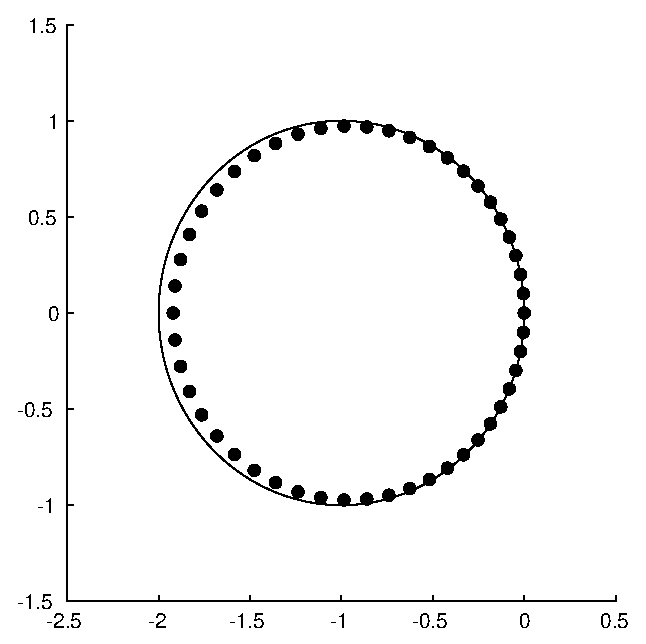
\includegraphics[width=0.95\linewidth]{figures/ex_12_82_mu=0.8.eps}
    \end{minipage}
    \begin{minipage}[t]{0.48\linewidth}
        \centering
        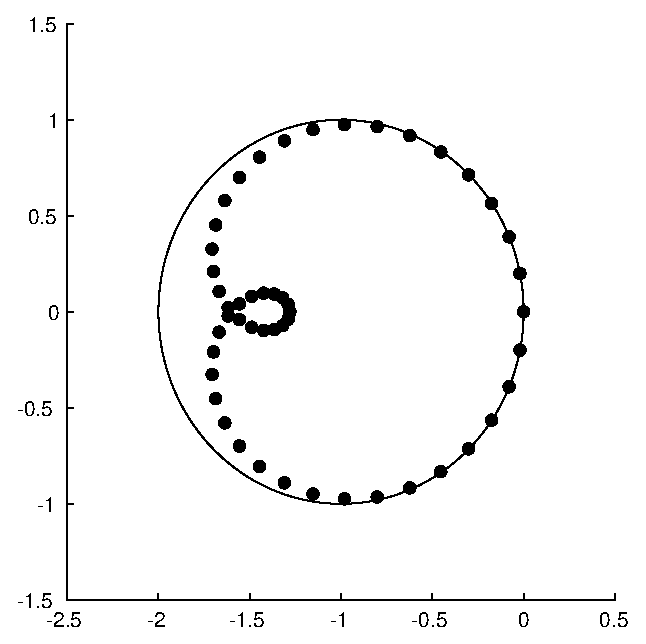
\includegraphics[width=0.95\linewidth]{figures/ex_12_82_mu=1.6.eps}
    \end{minipage}
    \begin{minipage}[t]{0.48\linewidth}
        \centering
        \vspace{.5em}
        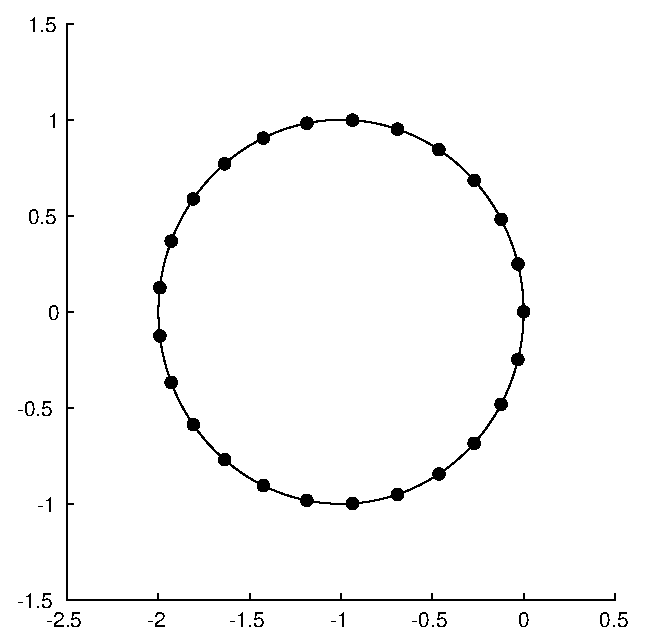
\includegraphics[width=0.95\linewidth]{figures/ex_12_82_mu=2.eps}
    \end{minipage}
    \begin{minipage}[t]{0.48\linewidth}
        \centering
        \vspace{.5em}
        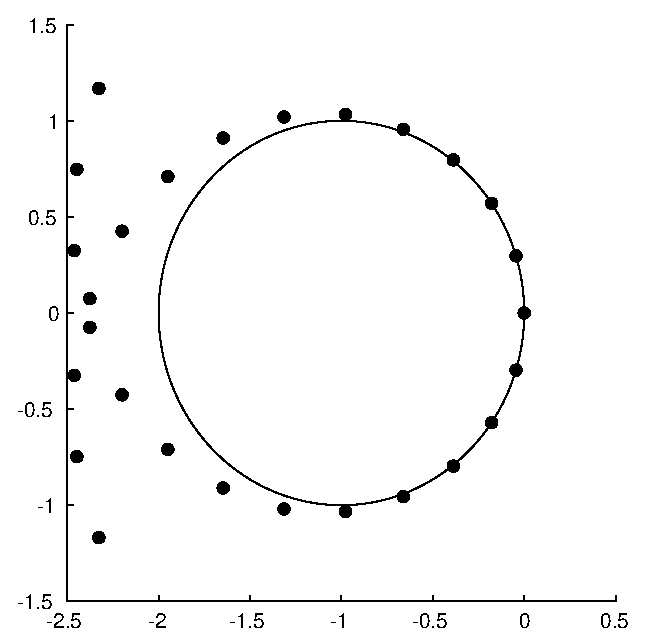
\includegraphics[width=0.95\linewidth]{figures/ex_12_82_mu=2.4.eps}
    \end{minipage}
\end{figure} \vspace{-.5em}

See the matlab code in \verb|ex_12_82.m|.

\section*{\large Exercise 12.86}

The numerical domains of dependence of the grid point $(x_j,t_3)$ for the upwind method with $a<0$ and $\mu=0$ is shown as the solid dots below.

\vspace{-.5em}
\begin{center}
    \begin{tikzpicture} 
        \draw[densely dashed][help lines] ( -2.401,0 ) grid[step=0.8cm] ( 2.4, 2.4);
        \fill (0,0) circle (2pt);
        \fill (0,0.8) circle (2pt);
        \fill (0,1.6) circle (2pt);
        \fill (0,2.4) circle (2pt);
        \coordinate [label=below:$x_j$] (A) at (0,0);
        \coordinate [label=left:$t_0$] (B) at (-2.4,0);
        \coordinate [label=left:$t_3$] (C) at (-2.4,2.4);
    \end{tikzpicture}
\end{center}

Also with $\mu=-1$.

\begin{center}
    \begin{tikzpicture} 
        \draw[densely dashed][help lines] ( -2.401,0 ) grid[step=0.8cm] ( 2.4, 2.4);
        \fill (2.4,0) circle (2pt);
        \fill (1.6,0.8) circle (2pt);
        \fill (0.8,1.6) circle (2pt);
        \fill (0,2.4) circle (2pt);
        \coordinate [label=below:$x_j$] (A) at (0,0);
        \coordinate [label=below:$x_{j+3}$] (D) at (2.4,0);
        \coordinate [label=left:$t_0$] (B) at (-2.4,0);
        \coordinate [label=left:$t_3$] (C) at (-2.4,2.4);
    \end{tikzpicture}
\end{center}

And with $\mu=-2$.

\begin{center}
    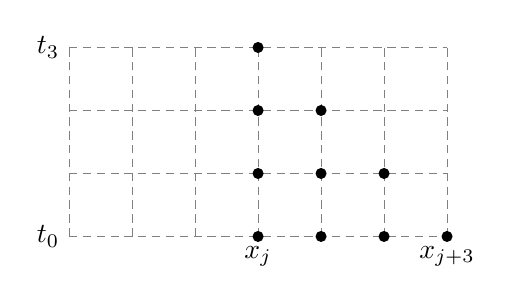
\begin{tikzpicture} 
        \draw[densely dashed][help lines] ( -2.401,0 ) grid[step=0.8cm] ( 2.4, 2.4);
        \fill (2.4,0) circle (2pt);
        \fill (1.6,0.8) circle (2pt);
        \fill (0.8,1.6) circle (2pt);
        \fill (0,2.4) circle (2pt);
        \fill (0,1.6) circle (2pt);
        \fill (0,0.8) circle (2pt);
        \fill (0,0) circle (2pt);
        \fill (0.8,0.8) circle (2pt);
        \fill (0.8,0) circle (2pt);
        \fill (1.6,0) circle (2pt);
        \coordinate [label=below:$x_j$] (A) at (0,0);
        \coordinate [label=below:$x_{j+3}$] (D) at (2.4,0);
        \coordinate [label=left:$t_0$] (B) at (-2.4,0);
        \coordinate [label=left:$t_3$] (C) at (-2.4,2.4);
    \end{tikzpicture}
\end{center}

\section*{\large Exercise 12.88}

When we fix $\mu=1$, (12.83) becomes
\begin{equation*}
    U_j^{n+1}=U_{j-1}^n.
\end{equation*}

The numerical domains of dependence of the grid point $(x_j,t_3)$ for the Lax-Wendroff method with $\mu=1$ is shown as the solid dots below.

\begin{center}
    \begin{tikzpicture} 
        \draw[densely dashed][help lines] ( -2.401,0 ) grid[step=0.8cm] ( 2.4, 2.4);
        \fill (-2.4,0) circle (2pt);
        \fill (-1.6,0.8) circle (2pt);
        \fill (-0.8,1.6) circle (2pt);
        \fill (0,2.4) circle (2pt);
        \coordinate [label=below:$x_j$] (A) at (0,0);
        \coordinate [label=below:$\;\;x_{j-3}$] (D) at (-2.4,0);
        \coordinate [label=left:$t_0\;$] (B) at (-2.4,0);
        \coordinate [label=left:$t_3\;$] (C) at (-2.4,2.4);
        \coordinate [label=right:$\;\;$] (BB) at (2.4,0);
    \end{tikzpicture}
\end{center}

Also with $\mu=-1$.

\begin{center}
    \begin{tikzpicture} 
        \draw[densely dashed][help lines] ( -2.401,0 ) grid[step=0.8cm] ( 2.4, 2.4);
        \fill (2.4,0) circle (2pt);
        \fill (1.6,0.8) circle (2pt);
        \fill (0.8,1.6) circle (2pt);
        \fill (0,2.4) circle (2pt);
        \coordinate [label=below:$x_j$] (A) at (0,0);
        \coordinate [label=below:$x_{j+3}$] (D) at (2.4,0);
        \coordinate [label=left:$t_0$] (B) at (-2.4,0);
        \coordinate [label=left:$t_3$] (C) at (-2.4,2.4);
    \end{tikzpicture}
\end{center}

\section*{\large Exercise 12.97}

First, replace $U_j^n$ with $v(x,t)$ and we have
\begin{equation*}
    \frac{v(x,t+k)-v(x,t-k)}{2k}=-\frac{a}{2h}(v(x+h,t)-v(x-h,t)).
\end{equation*}

Second, we expand all terms in Taylor series about $(x,t)$ to derive the modified equation as (for brevity, omit the dependence on $(x,t)$, and suppose $h=O(k)$)
\begin{equation}
    \frac{1}{2k}(2kv_t+\frac{1}{3}k^3v_{ttt})=-\frac{a}{2h}(2hv_x+\frac{1}{3}h^3v_{xxx})+O(k^4).
\end{equation}

Clearly we have
\begin{equation}
    v_t+av_x=O(k^2),
\end{equation}
which follows that
\begin{equation*}
    v_{ttt}+a^3v_{xxx}=O(k^2),
\end{equation*}

Substituting into (1) gives
\begin{equation*}
    v_t+av_x+\frac{ah^2}{6}(1-\mu^2)v_{xxx}=O(k^4),
\end{equation*}
which implies (12.95).

Now we retain one more term of higher-order derivative at step (1). And it gives
\begin{align}
    &\frac{1}{2k}(2kv_t+\frac{1}{3}k^3v_{ttt}+\frac{1}{60}k^5v_{ttttt}) \nonumber \\
    =& - \frac{a}{2h}(2hv_x+\frac{1}{3}h^3v_{xxx} + \frac{1}{60}h^5v_{xxxxx}) + O(k^6).
\end{align}

Follows from (2), we can easily get
\begin{align*}
    v_{tttxx}&=-a^3v_{xxxxx}+O(k^2),\\
    v_{ttttx}&=a^4v_{xxxxx}+O(k^2),\\
    v_{ttttt}&=-a^5v_{xxxxx}+O(k^2).
\end{align*}

Substituting into (3) gives
\begin{equation*}
    v_t+av_x+\frac{k^2}{6}v_{ttt}+\frac{ah^2}{6}v_{xxx}=C_1v_{xxxxx}+O(k^6),
\end{equation*}
where $C_1=O(k^4)$. Apply operator $\frac{\partial^2}{\partial t^2},\frac{\partial^2}{\partial t\partial x},\frac{\partial^2}{\partial x^2}$ to the above equation and combine the results. We can get
\begin{equation*}
    v_{ttt}+a^3v_{xxx}=C_2v_{xxxxx}+O(k^4),
\end{equation*}
where $C_2=O(k^2)$.

Substituting into (3) gives
\begin{equation*}
    v_t+av_x+\frac{ah^2}{6}(1-\mu^2)v_{xxx}=\epsilon_f v_{xxxxx}+O(k^6),
\end{equation*}
where $\epsilon_f=O(k^4)$. It implies (12.96).

If one more term of higher-order derivative is retained in the Lax-Wendroff method, we have
\begin{align}
    & v_t+\frac{k}{2}v_{tt}+\frac{k^2}{6}v_{ttt}+\frac{k^3}{24}v_{tttt}+a\left(v_x+\frac{h^2}{6}v_{xxx}\right) \nonumber\\
    =&\frac{k}{2}a^2v_{xx}+\frac{kh^2}{24}a^2v_{xxxx}+O(k^4).
\end{align}

Similarly we can get
\begin{equation*}
    v_{tt}-a^2v_{xx}=C_3v_{xxxx}+O(k^3),
\end{equation*}
where $C_3=O(k^2)$. And also we have
\begin{equation*}
    v_{tttt}=a^4v_{xxxx}+O(k).
\end{equation*}

Substituting into (4) gives
\begin{equation*}
    v_t+av_x+\frac{ah^2}{6}(1-\mu^2)v_{xxx}=\epsilon_w v_{xxxx}+O(k^4),
\end{equation*}
where $\epsilon_w=O(k^3)$. It implies (12.97).

\section*{\large Exercise 12.98}

First, replace $U_j^n$ with $v(x,t)$ and we have
\begin{align*}
    &\frac{v(x,t+k)-v(x,t)}{k}=-\frac{a}{2h}(3v(x,t)-4v(x-h,t)+\\& v(x-2h,t))+\frac{a^2k}{2h^2}(v(x,t)-2v(x-h,t)+v(x-2h,t)).
\end{align*}

Second, we expand all terms in Taylor series about $(x,t)$ to derive the modified equation as (for brevity, omit the dependence on $(x,t)$)
\begin{align*}
    &v_t+\frac{k}{2}v_{tt}+\frac{k^2}{6}v_{ttt}+O(k^3)=-\frac{a}{2h}(2hv_x-\frac{2}{3}h^3v_{xxx}+\\& O(h^4))+\frac{a^2k}{2h^2}(h^2v_{xx}-h^3v_{xxx}+O(h^4)).
\end{align*}

Assume $h=O(k)$ and it follows that
\begin{equation*}
    v_t+av_x=\frac{a^2}{2}kv_{xx}-\frac{k}{2}v_{tt}+(\frac{a}{3}h^2-\frac{a^2}{2}kh)v_{xxx}-\frac{k^2}{6}v_{ttt}+O(k^3).
\end{equation*}

Differentiate the above equation and we have
\begin{align*}
    v_{ttt}+av_{xtt}&=O(k),\\
    v_{ttx}+av_{xxt}&=O(k),\\
    v_{txx}+av_{xxx}&=O(k),\\
    v_{tt}+av_{xt}&=O(k^2),\\
    v_{tx}+av_{xx}&=O(k^2).
\end{align*}

Combining the above equations gives
\begin{equation*}
    v_t+av_x=(-\frac{1}{2}a^2kh+\frac{1}{6}a^3k^2+\frac{1}{3}ah^2)v_{xxx}+O(k^3).
\end{equation*}

Hence we have
\begin{equation*}
    v_t+av_x=\frac{ah^2}{6}(2-3\mu+\mu^2)v_{xxx}+O(k^3).
\end{equation*}
which implies (12.98). And by Example F.46, we have
\begin{align*}
C_p(\xi) &= a+\frac{ah^2}{6}(\mu-1)(\mu-2)\xi^2\\
C_g(\xi) &= a+\frac{ah^2}{2}(\mu-1)(\mu-2)\xi^2
\end{align*}

For $\mu\in(0,1)$, both $C_p$ and $C_g$ have a magnitude grater than $|a|$, hence numerical oscillations move ahead of the true wave crest. This answers Question (e) of Example 12.92.

\section*{\large Exercise 12.99}

The advection equation
\begin{equation*}
    \left\{
        \begin{array}{l}
            u_t+u_x=0,\\
            u(x,0)=\eta(x),
        \end{array}
    \right.
\end{equation*}
has the exact solution
\begin{equation*}
    u(x,t)=\eta(x-t).
\end{equation*}

If $\mu=1$, the Lax-Wendroff method gives
\begin{equation*}
    U_j^{n+1}=U_{j-1}^n.
\end{equation*}

Suppose $\mathbf{U}^n$ is exact, that is
\begin{equation*}
    U_{j-1}^n=u((j-1)h,nk)=\eta((j-1-n)k).
\end{equation*}

Then
\begin{equation*}
    U_{j}^{n+1}=U_{j-1}^n=\eta((j-1-n)k)=u(jh,(n+1)k).
\end{equation*}
which implies $\mathbf{U}^{n+1}$ is also exact. Hence the Lax-Wendroff method gives the exact solution at the grid points. Certainly better than the numerical solution with $k=0.8h$.

Similarly, if $\mu=1$ and suppose $\mathbf{U}^{n-1}, \mathbf{U}^n$ is exact, then the $\mathbf{U}^{n+1}$ given by the leapfrog method is also exact. This answers the Question (f) of Example 12.92.

\section*{\large Exercise 12.101}

Substituting $U_j^n=[g(\xi)]^ne^{\mathbf{i}\xi jh}$ into the Lax-Friedrichs method
\begin{equation*}
    U_j^{n+1}=\frac{1}{2}(U_{j+1}^n+U_{j-1}^n)-\frac{\mu}{2}(U_{j+1}^n-U_{j-1}^n)
\end{equation*}
gives
\begin{align*}
    g(\xi)&=\frac{1-\mu}{2}e^{\mathbf{i}\xi h} + \frac{1+\mu}{2}e^{-\mathbf{i}\xi h}\\
    &= \cos(\xi h) - \mathbf{i}\mu \sin(\xi h).
\end{align*}

Therefore
\begin{align*}
    |g(\xi)|^2&= \cos^2(\xi h) + \mu^2 \sin^2(\xi h)\\
    &= 1+(\mu^2-1)\sin^2(\xi h),
\end{align*}
and hence the method is stable provided $|\mu|\leq 1$.

\section*{\large Exercise 12.102}

Substituting $U_j^n=[g(\xi)]^ne^{\mathbf{i}\xi jh}$ into the Lax-Wendroff method
\begin{equation*}
    U_j^{n+1}=U_j^n - \frac{\mu}{2}(U_{j+1}^n-U_{j-1}^n) + \frac{\mu^2}{2}(U_{j+1}^n-2U_j^n+U_{j-1}^n)
\end{equation*}
gives
\begin{align*}
    g(\xi)&=1 - \frac{\mu}{2}(e^{\mathbf{i}\xi h}-e^{-\mathbf{i}\xi h}) + \frac{\mu^2}{2}(e^{\mathbf{i}\xi h}-2+e^{-\mathbf{i}\xi h})\\
    &= 1-\mathbf{i}\mu \sin(\xi h)-\mu^2+\mu^2\cos(\xi h)\\
    &= 1-2\mu^2\sin^2\frac{\xi h}{2} -\mathbf{i}\mu \sin(\xi h).
\end{align*}

Therefore
\begin{align*}
    |g(\xi)|^2&= \left(1-2\mu^2\sin^2\frac{\xi h}{2}\right)^2 + \mu^2 \sin^2(\xi h)\\
    &= 1+4\mu^2(\mu^2-1)\sin^4\frac{\xi h}{2},
\end{align*}
and hence the method is stable provided $|\mu|\leq 1$.

\end{document}
